\documentclass[output=paper]{langsci/langscibook} 
\author{%
Sascha Wolfer\affiliation{Institute for the German Language, Mannheim}
}
% \chapterDOI{} %will be filled in at production


\abstract{We present a study using eye-tracking-while-reading data from participants reading German jurisdictional texts. We are particularly interested in nominalisations. It can be shown that nominalisations are read significantly longer than other nouns and that this effect is quite strong. Furthermore, the results suggest that nouns are read faster in reformulated texts. In the reformulations, nominalisations were transformed into verbal structures. Reformulations did not lead to increased processing times of verbal constructions but reformulated texts were read faster overall. Where appropriate, results are compared to a previous study of \citet{Hansen2006} using the same texts but other methodology and statistical analysis. 
}
\title{The impact of nominalisations on the reading process: {A} case-study using the Freiburg Legalese Reading Corpus}
\rohead{The impact of nominalisations on the reading process}

\maketitle
\begin{document}

\section{Introduction}

In linguistics, text corpora are used to analyse rules and usage of language in natural contexts. Most of the time, corpora are annotated with linguistic information. These annotations allow linguists to search for recurring patterns and extract all instances of a specific linguistic structure from the corpus. These linguistic annotations can span several levels of linguistic structures (e.g., parts-of-speech and phrase structure). On the textual level, one might be interested in co-reference chains to investigate which words in the text refer to the same entity in the world. Some annotations can also be numerical in nature. One of the most common measures associated with words is the frequency with which the word occurs in natural language. Most of the time, a corpus itself is the source of this information. If one compiles a corpus of terminological language, however, the frequency of words in everyday language might also be interesting. Here, the source of the frequency information might well be another corpus.

In recent years, some researchers began to enrich corpora with another kind of annotation layer. If we collect or compile texts to create a corpus of natural language, we can take this corpus and show its contents to humans. Of course, these humans should be taken from a population likely to be confronted with the kind of text material we included in the corpus. The humans, who were exposed to our collected text material, are our readers. And while they are reading the text material, we can record their eye movements with an eye-tracker. In psycholinguistics, this method has been used for quite some time now. However, up until the last ten years or so, only carefully manipulated experimental stimuli were shown to readers. In psycholinguistic experiments, sentences might be constructed from scratch and only a single word could be exchanged for another to realise an experimental manipulation. Then, the effect of the experimental variation on processing behaviour is measured in form of reading variables (see \sectref{wolfer:sec:2.2} for a short introduction of reading variables). 

If we record eye movements on natural text (i.e., the corpus we constructed), we can add those eye movements as an additional annotation layer. Now, a specific word is not only associated with a certain frequency measure, part-of-speech information and the phrase it is located in. It now also has processing information associated with it. With such a ``reading corpus'', we have a powerful instrument at hand to investigate human reading of natural texts. The linguistic information can still be used to select specific instances from the corpus, but now we also know how humans processed these instances when they read them in the context of the whole corpus. Collection of eye-tracking data is expensive (in terms of scientific staff, participants and time). That is the reason why reading corpora are a lot smaller than text corpora we are used to in linguistics.

Several reading corpora are available in the field of psycholinguistics. Most of them are in English \citep{Frank2013, Kennedy2003}, but there are also reading corpora for French \citep{Kennedy2003} and German \citep{Kliegl2004, wolfer2013}. In this article, we present analyses based on the Freiburg Legalese Reading Corpus (FLRC), a corpus of jurisdictional terminological language. Jurisdictional language is known (at least in Germany) for its difficulties on several linguistic levels. \citet[170]{HansenSchirra2004} following \citet{Oksaar1988} and \citet{Wagner1981} identify the following linguistic properties as representative for jurisdictional language: long sentences, personalisations of inanimate objects or circumstances, complexity induced by derivations (the creation of new words with affixes), chains of subordinated nouns, extensive genitive attribution, archaic forms, formulaic expressions and nominalisations instead of verbs. We will focus on the last-mentioned structures: nominalisations. The overarching research questions will be: Are nominalisations really harder to process than other words (especially than nouns, which are most comparable)? And can nominalisations be reformulated effectively to make text processing less complex?

We will start out by presenting some arguments why jurisdictional language should also be understandable to lay people (§1.1). We will then describe some reading corpora in more detail (§1.2). Chapter 2 will introduce the Freiburg Legalese Reading Corpus and the linguistic information (§2.1) and eye-tracking data it contains (§2.2). In Chapter 3, we will present our data selection and preparation processes (§3.1), formulate the hypotheses (§3.2) and present the statistical analyses and results (§3.3). We will discuss these results in Chapter 4. Chapter 5 will conclude the article.

\subsection{\label{bkm:Ref283725774}Optimising the comprehensibility of jurisdictional language}

The linguistic inaccessibility of jurisdictional language stands in contrast to the highly relevant function the jurisdictional system fulfils in modern democracies. Jurisdictional texts of all kinds ensure peaceful coexistence in our society. In Germany, the Bundesverfassungsgericht (Federal Constitutional Court) plays a prominent role in the German jurisdictional system and in society as a whole. On a linguistic level, its decisions are highly complex and not easily understandable for their ultimate addressees, the citizens of Germany who are mainly lay people when it comes to interpreting jurisdictional texts \citep[cf. ][]{eichhoff2009denken}. Because of this prominent role of the Bundesverfassungsgericht, excerpts from decisions by this court were included into the reading corpus we are going to describe in this article. The corpus also contains full-length decisions. However, this part of the corpus will be of secondary interest in the present article. 

Of course, one could say that jurisdictional language does not have to be understandable to lay people because it is a language for special purposes or professional jargon just like the language of, for example, IT staff, miners or linguists. \citet{Towfigh2009} formulates such a position. There are (at least) two arguments against such a position. The professional jargons of IT people, miners or linguists are by far not as socially relevant as jurisdictional language. Of course, information technology also gets more important in modern social life. But still, it is far from being as important for the organisation of our social coexistence as jurisdictional language. If IT jargon might eventually get equally important, also the terminology of IT experts would face the demand of the public to get more understandable to everyone.

The second argument against the position that \citet{Towfigh2009}, amongst others, formulates is that even experts of the jurisdictional system struggle with their own professional code \citep[cf. ][]{eichhoff2009einstellungen}. As expected, 70\% of all 84 surveyed legal experts judge their professional code as ``weniger gut verständlich'' (not well comprehensible) for lay people. Another 26\% judge it as ``nicht verständlich'' (not comprehensible at all) for lay people \citep[138]{eichhoff2009einstellungen}. More surprisingly, though, 73\% of the legal experts have \textit{sometimes} trouble comprehending jurisdictional language themselves. Another 12\% state that they \textit{often} have trouble understanding jurisdictional language \citep[146]{eichhoff2009einstellungen}. The experts also largely agree that jurisdictional texts should be comprehensible for lay people without special training. Only 6\% of all experts do not agree to this statement \citep[139]{eichhoff2009einstellungen}.

So, the demand for easier comprehensible jurisdictional language is formulated both by lay people and legal experts. With this motivation in mind, we compiled the Freiburg Legalese Reading Corpus. We wanted to provide detailed empirical data on the comprehension process of jurisdictional language. In terms of internal/external validity, we tried to make a compromise within Freiburg Legalese Reading Corpus: The part of the corpus with reformulations is clearly more similar to the classic psycholinguistic experiment because excerpts from original court decisions were reformulated by linguists making at least the reformulations not ecologically valid anymore. The other part of the corpus contains complete texts that were not altered. So, this part of the corpus can be considered ecologically more valid.

With this empirical data, hypotheses regarding the processing of specific linguistic constructions can be tested. We chose not to construct the linguistic stimuli from scratch but to use real-life linguistic stimuli. We hope that insights gained from these analyses can be generalised to other real-life texts. In empirical terms, we aimed for high ecological validity. 

\subsection{\label{bkm:Ref283725832}Reading corpora}

As already outlined in the introduction, research using reading corpora has gained increasing influence in psycholinguistics and related disciplines. Reading corpora are large collections of eye-tracking data on text material. There are already several reading corpora available in the field: The English UCL Corpus \citep{Frank2013} contains eye-tracking and self-paced reading data. The German Potsdam Sentence Corpus (PSC, \citealt{Kliegl2006}) consists of artificial sentences constructed around target words. These target words were selected for word class (noun or verb), frequency (high or low) and length (short, medium or long). For each of the 12 combinations of these factors, 12 sentences were constructed, leading to a total of 144 sentences. Please keep in mind that these sentences never occurred in the real world and are not connected to each other on a content level. The English/French Dundee Corpus \citep{Kennedy2003} contains editorials from \textit{The Independent }and \textit{Le Monde}. Recently, the PopSci corpus with German popular science texts has been introduced to the field \citep{MuellerFeldmeth2013}. Here, 16 texts from popular science journals are contained in the text corpus and were read by human readers. So, connections between sentences on a textual level (e.g., co-reference chains) were still intact.

One of the first applications of reading corpora has been the evaluation of models of eye-movement control. There is still a considerable debate in this field, mainly between two models, the E-Z Reader \citep{Reichle2003} and the SWIFT \citep{Engbert2005} model. Fairly low-level processes are the focus of both computational models. The models are mainly interested in when and where a reader moves the eyes while reading text. These low-level processes have to be considered, of course, but are not the primary focus of this chapter. Recently, higher-level processes in language comprehension have come to the attention of researchers using reading corpora. Several psycholinguistic models and theories have been investigated and evaluated using reading corpora: Surprisal \citep{Demberg2008, Patil2009} cue-based parsing and similarity-based interference \citep{MuellerFeldmeth2013}; semantic constraint \citep{Pynte2008} and many more. In this article, we are going to investigate research questions dealing with the lexical level. Namely, we are going to analyse the processing of nominalisations and how, if at all, they can be reformulated.

\section{\label{bkm:Ref283224577}The Freiburg Legalese Reading Corpus}

All data for the Freiburg Legalese Reading Corpus was collected in the eye-tracking labs of the Centre for Cognitive Science at the University of Freiburg.

\subsection{\label{wolfer:sec:2.1}Language material}

The Freiburg Legalese Reading Corpus consists of two main parts: (1) A sub-corpus with nine original full length texts (three decisions, three press releases, and three newspaper articles) and (2) a sub-corpus containing thirty short sections of original decisions with thirty moderately reformulated texts and thirty strongly reformulated texts. The first part consisting of full-length texts has 12,769 tokens. The second part with excerpts from decisions and the associated reformulations has 2,898 tokens. In the analyses, we will use data from both corpus parts but will focus on the second part (excerpts and reformulations) later on.



\begin{table}
\begin{tabularx}{\textwidth}{XXXX} & Nominalisations & Complex NPs & Syntax\\
\lsptoprule
 Original excerpts & 10 texts\newline  200 tokens & 10 texts\newline  303 tokens & 10 texts\newline  434 tokens\\ \\
 \raggedright Moderate reformulations & 10 texts\newline  214 tokens & 10 texts\newline  317 tokens & 10 texts\newline  439 tokens\\ \\
\raggedright  Strong reformulations & 10 texts\newline  217 tokens & 10 texts\newline  334 tokens & 10 texts\newline  440 tokens\\
\lspbottomrule
\end{tabularx}
\caption{Corpus design of the corpus part with the original excerpts and reformulations. Total token counts of the 10 texts in each cell are also shown. Column names are the three complexity types \citet{Hansen2006} used to select the original excerpts.}
\label{wolfer:tab:1}
\end{table}

The excerpts and reformulations are especially useful for the analysis at hand. See \tabref{wolfer:tab:1} for a brief overview over the design of this corpus part. The thirty original excerpts were selected to meet one of three types of linguistic complexity (henceforth ``complexity type''). Ten texts contain many nominalisations that were transformed into verbal structures during the course of reformulation (complexity type ``nominalisations''). Ten texts contain very complex noun phrases – mostly due to excessive pre- or post-nominal modification (complexity type ``complex NPs''). In the first reformulation step, these modifications were transformed into subordinate clauses. In the second step leading to the strongly reformulated version, sentences were split to avoid the sentential complexity induced by these subordinate sentences. The remaining ten original texts contained very long and multiply embedded sentences (complexity type ``syntax''). They were split up repeatedly to achieve the moderately and strongly reformulated versions. All texts, including the reformulated versions, were taken from a study of \citet{Hansen2006}. They reformulated the texts with the help of a jurisdictional expert who made sure that semantic content of the texts was maintained. Annotations of the texts were added by two student assistant annotators with the help of the software ``Annotate'' \citep{Plaehn1998} for semi-automatic syntactic annotation. Parts-of-speech according to the Stuttgart-Tübingen-TagSet\footnote{The tag table is available under \url{http://www.ims.uni-stuttgart.de/forschung/ressourcen/lexika/TagSets/stts-table.html} (Accessed 2014-12-23)} and phrase structure were annotated. ``Annotate'' makes suggestions for both and the annotators altered these annotations in case they were incorrect. When the annotators did not agree on a certain annotation, agreement was established through discussion. Nominalisations were identified manually.

Example 1 shows an original excerpt from the complexity type ``nominalisations'' (1a) and the associated strongly reformulated text (1b)\footnote{The English meaning of this excerpt is: More than twelve years after Germany was re-united, the authorisation to reduce or repeal the reduction of fees by legal decree has been condensed to a legal duty to repeal the partial payment of fees.}. From Example 1a, the original excerpt, in transition to Example 1b, the strong reformulation, \citet{Hansen2006} transformed four *ung-nominalisations (``Herstellung'', ``Reduzierung'', ``Aufhebung'', ``Aufhebung'') into verbal structures (``hergestellt wurde'', ``reduziert/aufgehoben wird'', ``aufzuheben'').

Mehr als zwölf Jahre nach der Herstellung der deutschen Einheit habe sich die Ermächtigung zur Reduzierung oder Aufhebung der Gebührenermäßigung durch Rechtsverordnung zu einer Rechtspflicht zur Aufhebung des Gebührenabschlags verdichtet.

More than twelve years after the making of\_the German unity had itself the authorization to reduction or reversal theGEN reduction\_of\_fees through legal\_decree to a legal\_duty to\_the reversal theGEN partial\_payment\_of\_fees condensed.

Mehr als zwölf Jahre nachdem die deutsche Einheit hergestellt wurde, habe sich die Ermächtigung, dass die Gebührenermäßigung durch Rechtsverordnung reduziert oder aufgehoben wird, zu der Rechtspflicht   verdichtet, den Gebührenabschlag aufzuheben.

More than twelve years after the German unity   realised been, had itself the authorization, that the reduction\_of\_fees through legal\_decree reduced or abolished isAUX, to the legal\_duty condensed the partial\_payment\_of\_fees abolish.

As already mentioned above, this does not change the semantic content of the text. Example 1 is a typical example in terms of reformulations of nominalisations. The frequently used nominalisations are transformed into verbal structures. However, as can also be seen in Example 1, subordinating structures have to be introduced to integrate these newly introduced verbal structures in the sentence context. These subordinating structures can be identified by the subordinating conjunctions ``nachdem'' and ``dass'' in Example 1b. Only nouns ending with \textit{--ung} are treated as nominalisations in the remainder of this article.

When we analyse all 30 texts within the complexity type nominalisations (first column in \tabref{wolfer:tab:1}), we see that the share of nominalisations in all words drops significantly from 16.8~\% (originals) to 10.6~\% (moderate reformulations) and 10.5~\% (strong reformulations). Raw numbers for all 10 texts in each cell taken together are 35 (originals), 23 (moderate reformulations) and 23 (strong reformulations) nominalisations. So, obviously, no nominalisations were reformulated during the second step of the reformulation process\footnote{For some of the texts, \citet{Hansen2006} did not create a strongly reformulated version.}. To measure the impact of reformulations on the use of verbal structures, we sum up all occurrences of verbs and participles and look at the development of shares and raw figures over the reformulation versions. The verbal structures follow the opposite pattern of nominalisations. The share of verbal structures in all words rises significantly from 9.7~\% (originals) to 20.0~\% (moderate reformulations) and 21.1~\% (strong reformulations). Again, most of the reformulations are obviously going on between the originals and the moderate reformulations. The raw figures confirm this. The original texts contain 18, the moderately reformulated texts 41 and the strongly reformulated versions 45 verbs and/or participles. In the remainder of this chapter, we will investigate which influences these reformulations have on the reading process.

\subsection{\label{wolfer:sec:2.2}Eye-tracking data}

All texts were distributed on pages that matched a 20-inch-flatscreen with a resolution of 1600 by 1200 pixels. Texts were presented in a 48 pt proportional serif font to allow for as natural as possible a reading experience. A maximum of 11 lines of text with 1.5 line spacing fit on one screen page. After each text, a comprehension question had to be answered by pressing `yes' or `no' on a response box. Questions were rather easy and were primarily included into the study to keep participants attentive. We used an SR Research EyeLink 1000 for data collection. The eye-tracker measured gaze position of the participants with a rate of 1000 Hz which produces 1 data point every millisecond. Calibration and validation was carried out before the experiment and – if necessary – data collection was interrupted to recalibrate the eye-tracker.

Reading data was collected from 80 human readers (40 for each corpus part) who were given course credit or monetary compensation for their participation. Participants were all students at the University of Freiburg with normal (56 participants) or corrected vision (24 participants). Data on the age of participants was not gathered. It was made sure that none of the participants had an educational background in law. 51 participants were female. Participants were seated with their heads on a chin rest, so that their eyes were approximately 60 cm away from the screen.

Reading time variables were calculated with custom R \citep{R2014} scripts from the fixation data collected and pre-calculated by the eye-tracker's data export tool (SR Research DataViewer). For the identification of fixations, we used the default parameter settings of DataViewer. Each fixation was associated to an interest area. Interest areas spanned individual words and were expanded vertically to the middle of the space between lines. Fixations not associated with an interest area were discarded.

The following reading variables can be considered standard measures in psycholinguistic reading research and were pre-computed for all words in the corpus: First fixation duration (the duration in milliseconds of the first fixation on the current word), first-pass reading times (the summed duration of all fixations from entering the word until exiting the word to the left or to the right), regression path durations (the summed duration of all fixations from entering the word until a word right of the word is fixated, including all fixations on material left of the word, i.e. regressions) and total reading times (the summed duration of all fixations on the word, also including fixations after the word has been exited to the right for the first time, i.e. if the reader re-reads the word later on). Several more reading variables can be calculated from these measures. For example, re-reading time (total reading time minus first-pass reading time) or a binary variable if a regressive saccade has been launched during the first reading of a word (is the regression path duration longer than the first-pass reading time?). Another variable that is frequently used is skipping probability that is derived from a binary variable if a word is read during first pass (is the first-pass reading time greater than zero?). Considering the whole FLRC, mean first fixation duration was 200 msec. Mean first-pass reading time was 265 msec. Mean regression path durations were 495 msec. Mean total reading times were 405 msec. On average, a regressive saccade was launched on 12.6\% of all words in the FLRC. 

We will not go into much detail regarding the cognitive processes associated with each of these reading time variables. This has been excellently done elsewhere in much more detail \citep{Clifton2007, Hyona2003, Rayner2006}. A few words have to be said, though. First-pass reading times include all fixations during reading a region of interest (here, regions of interest are words) for the first time. First-pass reading times therefore capture processes of word recognition and early stages of word processing. Regression path duration or go-past time, as it is also called, ``can reasonably be construed as the time it takes upon reading the target word on first pass until it is successfully integrated with the on-going context'' \citep[620]{Rayner2006}. This, however, should not be the main problem of processing nominalisations. Of course, nominalisations have to be integrated into the context of the sentence – just as any other noun. However, we expect that the specific problem of processing a nominalisation is lexical, and not one of integration into the previous sentence context. So, we expect effects of nominalisations in rather early measures (e.g., first-pass reading time) and not in regression path durations. If we indeed find an effect in regression path durations and the probability of launching a regressive saccade upon encountering a nominalisation, this may be a hint that nominalisations are indeed harder to integrate into the previous context than normal nouns. An effect in total reading times cannot be ruled out because nominalisation may also be revisited after first pass.

\section{\label{bkm:Ref283726002}The impact of nominalisations on the reading process}

Nominalisations can be considered complex for two reasons. \citet{Hansen2006} describe them as an instrument to increase the informational density in a text: ``Information is packed into heavy noun phrases and nominalisations rather than being distributed onto larger grammatical units [\ldots]'' (ibd., p. 24). Also, nominalisations can be used to create constructions like ``die Abschiebung wird durchgeführt'' (the deportation is carried out). Such constructions enable objective and pertinent descriptions (``objektive und sachbezogene Darstellung``, \citealt[169]{HansenSchirra2004}) without mentioning a specific agent of the action. This may be odd for lay people and may lead to comprehension difficulties because such agent-less constructions are not very common in every-day language but rather have to be considered a property often found in terminological language \citep[cf. ][170]{HansenSchirra2004}. 

Given the previously introduced linguistic material and the corresponding processing data, we are able to investigate several questions. The most obvious question is: Is it difficult to process nominalisations? This, however, is not a valid research question because no linguistic entity is mentioned to which nominalisations are compared. We will start by comparing nominalisations to all other nouns. We will then also compare the size of the effect nominalisations have on the reading process with the effects of other word classes (content/function words, finite verbs, all nouns). With this comparison, we want to estimate the relative size of the effect that nominalisations have on the reading process.

We will then go into detail using the part of the reading corpus that contains excerpts and reformulations. Ten texts were specifically selected because they contain many nominalisations. Those texts were reformulated in two steps. We will therefore check if the reformulations generally slow down the processing of verbs and participles. The final questions will be if overall text processing benefits from the reformulations of nominalisations. All research questions are also summarised in the first column of \tabref{wolfer:tab:2}.

\subsection{\label{wolfer:sec:3.1}Data selection and preparation}

Each research question posed above needs a specific subset of the reading corpus to be answered. The data subsets associated with the respective research questions can be found in the second column of \tabref{wolfer:tab:2}.

\begin{table}
\begin{tabularx}{\textwidth}{XXX}
\lsptoprule
 Research question & Data subset & Hypothesis\\
\midrule 
 Are nominalisations harder to process than normal nouns? & All nouns (including nominalisations) in the FLRC & Nominalisations are read longer during first-pass.\\ \\
 How pronounced is the nominalisation effect compared to other classes of words? & All words in the FLRC & Compared to other word classes, the nominalisation effect is rather large.\\ \\
 Are nouns read faster after nominalisations have been reformulated? & All nouns in complexity type nominalisations & Nouns are read faster after nominalisations have been transferred to verbal structures.\\ \\
 Do reformulations shift complexity to verbal structures? & Verbs and participles in complexity type nominalisations & No observable effect\\ \\
 Does overall text processing benefit from the reformulations? & Whole texts of complexity type nominalisations & Reformulated texts are processed faster than original excerpts.\\
\lspbottomrule
\end{tabularx}
\caption{Research questions, selected data subsets, and hypotheses for the analyses presented in this chapter}
\label{wolfer:tab:2}
\end{table}
After the respective data subset has been selected from the reading corpus, we have to control for some effects that are rather obvious but not interesting for the research questions at hand. For example, it is common sense that longer words take longer to read. Also, it has been shown repeatedly that corpus frequency is a good predictor for reading times. The more frequent the actual word (hitherto: word \textit{n}) is encountered in natural language, the faster it is read \citep[cf. ][]{Kliegl2004}. This frequency effect extends to bigram and trigram frequencies, the corpus frequency of word \textit{n }in combination with words \textit{n }– 1 and, for trigrams, \textit{n – }2 \citep[cf. ][]{Boston2008}. Another factor that plays a crucial role for reading times is orthographic familiarity. Orthographic familiarity is a measure of how often a specific word shape appears in the language \citep[cf. ][]{White2008}. Orthographic familiarity is operationalised by the cumulative frequency of all words with the same initial three letters and the same length as the critical word. 

On the syntactic level, the position of word \textit{n} in the sentence and its depth of embedding in the phrase structure are relevant predictors for reading times \citep[cf. ][]{Pynte2008}. Words that occur later in the sentence are read faster. The same holds for words that are embedded deeper in the syntactic structure.

Other factors that can influence the reading times of words are related to the presentation of the words on the screen. The position of the text on the screen is relevant because, generally speaking, words appearing ``later'' on the screen are read faster. Also, reading behaviour on first and last words in lines can deviate from standard reading behaviour within a line. This is especially true for the first word in a row because it is the first word that is encountered after a change of text lines. If a reader changes the line, she or he has to initiate a very long saccade from the end of the line to the beginning of the next line. The fixation following this long saccade tends to be longer.

We control for all these factors by including the relevant variables word length, unigram, bigram and trigram frequencies, orthographic familiarity, position in the sentence, depth of embedding and presentation factors in statistical baseline models\footnote{The statistical baseline models are quite extensive and can be requested from the author. All models in the current article were fitted using linear mixed-effects models within the statistical environment R \citep{R2014} and the package lme4 \citep{Bates2014}.}. Participant and text identity were included as random intercepts into the models. When we analyse the effect of nominalisation, for example, the effect of the word's frequency is controlled for beforehand. This is desirable because, on the one hand, it reduces noise in our data and could lead to more pronounced effects of the factors we are interested in. On the other hand, this procedure also makes sure that variance in reading times that is really explained by word frequency or another control factor is not erroneously ascribed to other effects. Intuitively, the procedure leads to ``cleaner'' data and more reliable models. 

\subsection{\label{bkm:Ref283726131}Hypotheses}

All hypotheses can also be seen in the third column of \tabref{wolfer:tab:2}. If nominalisations are indeed more complex than normal nouns, we expect elevated first-pass (and eventually total) reading times for nominalisations compared to normal nouns. We would not necessarily expect an effect in regression path durations because the main problem of nominalisations should be a lexical one and not to integrate the nominalisations into the sentence context. At least, this should not be more of a problem than for normal nouns. When we compare the effect of nominalisations to the effects of other word classes, we would expect that the nominalisation effect is rather large. One could say that, the larger the nominalisation effect is in comparison to other effects, the more important it is to reformulate nominalisations or not to introduce them into texts in the first place. We will evaluate these first two hypotheses in the first section of the results section.

Regarding the reformulations, we would expect nouns to be read faster after nominalisations have been reformulated. This should simply be the case because the share of nominalisations in all nouns gets lower in reformulated texts (see \sectref{wolfer:sec:2.1} for statistics on the linguistic consequences of reformulations). The effect should be observable for first-pass (and eventually) total reading times.

We would also expect – if the reformulations were successful – that complexity is not simply shifted to another linguistic level or towards other linguistic structures, namely verbs and participles (see \sectref{wolfer:sec:2.1} for the relationship between reformulations and verbs and participles). If reformulations do not slow down processing of verbal structures, we do not expect an effect of reformulations on the reading times of verbs and participles. We will evaluate the latter three hypotheses in the second section of the results section.

For the last research question, we move away from the level of single words and take the whole texts of the complexity type nominalisations into account. This is a rather coarse grained measure that cannot tell us anything about the processing of single words. However, we can investigate the overall time it needs to process the original and reformulated texts as a whole. If reformulations were successful also on the textual level, we would expect slightly reduced reading times for the whole text for the reformulated versions.

\subsection{\label{bkm:Ref283726141}Results}

In this section, the research questions and associated hypotheses are categorised into two groups. The first group of research questions relates to the complexity of nominalisations in the whole reading corpus and the comparison to other word classes. The second group of research questions deals with the consequences it has on text processing when nominalisations are reformulated. 

\subsubsection{Complexity of nominalisations}

For the first research questions, all nouns in the reading corpus were selected. Each of those nouns is associated with the information if it is a nominalisation or not. This is the only predictor we include into our model as a fixed effect. We calculated linear mixed-effects models for the reading time variables first-pass reading time, total reading time and regression path durations. Those reading time variables were corrected by the baseline model procedure introduced in \sectref{wolfer:sec:3.1} For skipping probability and the probability that a regressive saccade is launched upon encountering the noun, logistic mixed regression models were calculated. These models are better suited for binary outcome variables \citep[cf. ][]{Jaeger2008}.

\begin{table}
\begin{tabularx}{\textwidth}{Xrrr}
\lsptoprule
 & Estimate & Standard Error & \textit{t}/\textit{z} value\\
\midrule 
 First-pass reading times & 0.063 & 0.012 & 5.243\\
 Total reading times & 0.131 & 0.015 & 8.911\\
 Regression path durations & 0.073 & 0.020 & 3.615\\
 Probability of being skipped & {}-0.536 & 0.033 & {}-16.087\\
\textit{p} {\textless} .0001\\
 Probability that a regressive saccade is launched & 0.059 & 0.035 & 1.662\\
\textit{p} = 0.10\\
\lspbottomrule
\end{tabularx}
\caption{Model parameters (estimate, standard error and t value) for the fixed effect of a noun being a nominalisation. The five models for the different reading variables are in rows. P values are only available for the logistic mixed regression models for skipping probability and the probability of a regressive saccade (last two rows). For all other models, an absolute t value above 2 strongly indicates significance. The sign of the estimate indicates the effect direction.}
\label{wolfer:tab:3}
\end{table}
3 shows the model parameters for this first analysis. First-pass reading times, total reading times and also regression path durations are significantly higher for nouns that are nominalisations than for normal nouns. Please bear in mind that the effects for the reading time variables cannot simply be ascribed to word length (nominalisations are likely to be longer than normal nouns) because the baseline modelling rules this out beforehand. The probability of being skipped is significantly lower for nominalisations. The probability that a regressive saccade is launched upon encountering a nominalisation is \textit{not} significantly higher than for normal nouns. This is somewhat surprising because the regression path durations are significantly higher for nominalisations. A likely explanation would be that first-pass reading times are also included in regression path durations and that the effect in regression path durations are really ascribable to the effect in first-pass reading times. So, we can conclude that nominalisations do not trigger more regressions back into previous text material than normal nouns. This relates to the question if nominalisations may also be harder to integrate into the sentence context than normal nouns. Given the results in \tabref{wolfer:tab:3}, this does not seem to be the case. Nevertheless, the impact of nominalisations on context integration processes needs to be further investigated to tease apart these effects.

 
\begin{figure}
 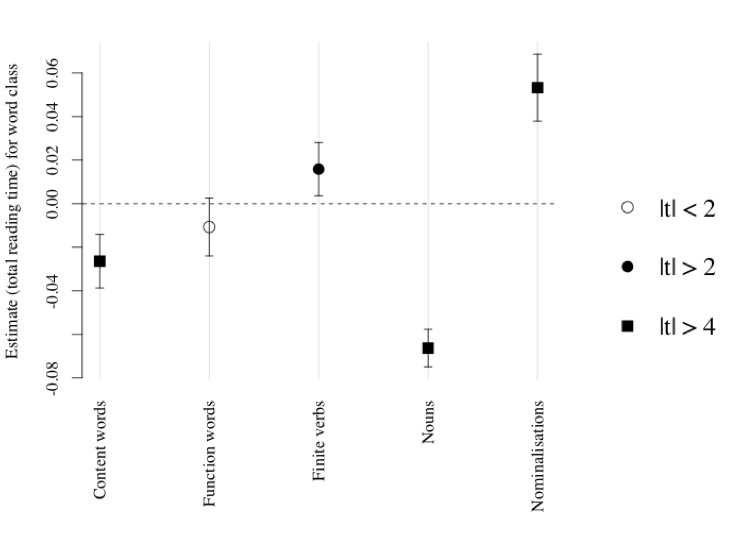
\includegraphics[width=\textwidth]{figures/Wolfer1.png}
\caption{Comparison of effects estimates (y axis) for total reading times and the effects of being a content word, function word, finite verb, noun or nominalisation. The associated t value is symbolized by the plot symbols.}
 \label{wolfer:fig:1}
\end{figure} 


With the next analysis, we are comparing the nominalisation effect to other sets of words. We will concentrate on total reading times here, because the most pronounced effect was shown for this variable (second row of \tabref{wolfer:tab:3}). We are going to compare the effect estimates because this model parameter can be thought of as an operationalisation of the effect strength\footnote{In simple linear regression with only one predictor variable, the estimate is the slope of the regression line.}. We include all words in the reading corpus into this analysis. For each word, we code if it belongs to one or more of the following set of words: content words, function words, finite verbs, nouns, nominalisations. We chose finite verbs as a set for comparison because finite verbs most of the time encode the main action going on in a sentence and should be considered quite relevant. With this coding, it is clear that each nominalisation belongs not only to the set of nominalisations but are also a subset of content words and nouns. 

All those declarations that are either TRUE or FALSE for each word then enter one linear mixed-effects model as fixed effects. By comparing the estimates for the fixed effects, we get an impression of the relative importance of these estimates. The estimates are visualised in \figref{wolfer:fig:1}. We are especially interested in the right-most point, the effect estimate for nominalisations. The estimate (\textit{$\beta $} = 0.053, \textit{t} = 6.80) is relatively high compared to all other effect estimates. This means that total reading times on a word are much higher when it is a nominalisation. This is surprising when we compare this estimate with the one for all nouns. The relatively low estimate (\textit{$\beta $} = -0.066, \textit{t} = -15.15) for nouns means that, if a word is a noun, total reading times on this word are much lower than for all other words. It can also be seen that the effect for nominalisations seems to be way stronger than the one for finite verbs (\textit{$\beta $} = 0.016, \textit{t} = 2.55) which have to be considered quite important elements in sentences.

\subsubsection{Consequences of reformulating nominalisations}

The results for the analyses of reformulations do not seem to be as clear as the ones introduced in the last chapter. If we use the reading times for the baseline models, no significant effects can be shown. All differences go into the right direction here (nouns are read faster in reformulated versions) but there seems to be too little power in the data to show significant effects here. If we only include word length, word frequency, word familiarity and presentation factors (see \sectref{wolfer:sec:3.1} for an explanation of these variables), we can show a significant effect of reformulation. Since most of the reformulation is going on between the original excerpts and the moderately reformulated versions, we treat both moderately and strongly reformulated versions as ``reformulated''. This way, we only have the contrast between nouns in original and nouns in reformulated texts. This makes the model parameters interpretable more easily. The model shows that nouns in reformulated texts are indeed read faster. This time, we only find a significant effect for first-pass reading times (\textit{$\beta $} = -0.076, \textit{t} = -2.05) but not for total reading times (\textit{$\beta $} = -0.080, \textit{t} = -1.22).

The next question is if processing complexity shifts to verbs and participles when nominalisations are reformulated. For this analysis, we selected all verbs and participles\footnote{In the tag set we used, verbs and participles are all words from one of the following parts-of-speech: VAFIN, VMFIN, VVINF, VVFIN, VVIZU, VAINF, VVPP, VMPP, VAPP.}{ }from the texts of complexity type ``nominalisations''. Verbs and participles were selected because nominalisations were transformed into verbal structures (see Example 1). It would be unfortunate for reformulation efforts if processing complexity simply shifts to the ``substitute structures'' that are introduced when nominalisations are reformulated (also see \tabref{wolfer:tab:2}). No effects can be shown for either first-pass reading times (\textit{$\beta $} = -0.011, \textit{t} = -0.20) or total reading times (\textit{$\beta $} = -0.106, \textit{t} = -1.65) and all effect estimates point into the negative direction, i.e. verbs and participles are read slightly (and not significantly) \textit{faster}. Please note, if no effect can be shown, this does not mean that there really is no effect. It could always be the case that we simply cannot \textit{detect} the effect. However, if reformulations really would lead to increased reading times on verbs and participles because these were the structures that were introduced by transforming nominalisations, then the reading times in the reformulated version should be \textit{higher}, which is not the case. 

To answer the last question, we take the analyses to the text level and compare the reading times of the different reformulation versions of the texts from the complexity type nominalisations. Indeed, as \tabref{wolfer:tab:4} shows, the mean reading time per text is getting lower as texts are reformulated. However, the noise (standard deviations, second column) is also very high here. Apart from that, we also have to take text length into account, because it is not that big of a surprise that texts are read faster if they are shorter. Indeed, they get a little shorter in average as the third column of \tabref{wolfer:tab:4} shows.
\begin{table}
\begin{tabularx}{\textwidth}{lXXX} 
& Mean text\newline reading time & Standard \newline deviation & Mean text \newline length\\
\lsptoprule
 Original excerpts & 9489 ms & 7607 ms & 149 characters\\
 Moderate reformulations & 8487 ms & 7748 ms & 144 characters\\
 Strong reformulations & 8018 ms & 6193 ms & 143 characters\\
\lspbottomrule
\end{tabularx}
\caption{Mean text reading times, standard deviations and mean text lengths for text from the complexity type nominalisations}
\label{wolfer:tab:4}
\end{table}
To tease apart the effect of text length and relate the noise to the effect, we have to calculate a statistical model. Reformulation version and text length (as a control factor) are entered as fixed effects and participants and text identity are treated as random intercepts. We predict the logarithm of text reading time\footnote{The effects I report are even more pronounced when raw text reading time is predicted. However, it is statistically more appropriate to predict logarithmized text reading times because they follow a normal distribution more closely than raw text reading times.}. As expected, there is a clear effect of text length on text reading time (\textit{$\beta $} = 0.006, \textit{t} = 5.16), texts are read longer when they contain more characters. Apart from that, the effect we are interested in is also significant and it points into the direction the hypothesis suggests. Strongly reformulated texts are read faster than the original excerpts (\textit{$\beta $} = -0.157, \textit{t} = -2.58). Moderately reformulated texts, however, lie somewhere in between the originals and the strong reformulations (\textit{$\beta $} = -0.109, \textit{t} = -1.79) and are not significantly different from either one of them in terms of text reading time. Again, this does not replicate the findings of \citet{Hansen2006}. There are several possible reasons for this: (1) I used a different method to measure text reading time. We summed all total reading times of all words. \citet{Hansen2006} measured the time between text presentation on-set till participants advanced to the question. (2) Hansen et al. did not correct for text length when estimating reading times. (3) Also, to our knowledge, they did not include random intercepts for participants and/or text identity. That means that inter-individual differences (between texts and/or participants) are not accounted for.\label{bkm:Ref283726149} (4) Hansen and colleagues analyse reading time differences over all complexity types while I only analysed texts of the complexity type ``nominalisations'' because these are the texts relevant for the current research question. 

\section{Discussion}

All hypotheses mentioned in the third column of \tabref{wolfer:tab:2} were confirmed by the statistical analyses. Indeed, nouns, which are nominalisations, are read slower. This is confirmed by significant effects for first-pass reading times and total reading times. Also, nominalisations are less likely to be skipped. Although nouns in general are read faster than all other words in the reading corpus, this effect is the other way around for nominalisations. The effect size for nominalisation (i.e. the impact on the reading process) is comparable and even higher than the same effect for finite verbs.

So, nominalisations really seem to be quite complex for the reader to process. However, we also showed that – at least in our reformulation corpus – they can be reformulated. In the reformulated versions of the original excerpts, nominalisations were transformed into verbal structures. When comparing the reading times of nouns in the original versions with those in the reformulated versions, we found significantly faster reading on all nouns. It also does not seem to be some kind of trade-off where we just switch complexity introduced by nominalisations for complexity on verbs and participles. Those did not seem to be read longer in reformulated text versions. When using the very rough measure of overall text reading time, we saw that reformulated texts are read slightly faster. So, although nominalisations indeed seem to introduce a fair bit of complexity into jurisdictional texts, they obviously can be reformulated without just shifting processing complexity to another linguistic level.

However, we still have to bring these results into line with the larger context of text processing and text comprehension. It has been shown during the course of this article that nominalisations take longer to process and this is a quite pronounced effect. However, we did not present any data on the consequences for the mental representation the participants built up while reading the texts. Such consequences could be measured by asking participants to answer questions after reading the texts. This also has been done during data collection for the FLRC. We used the same questions like \citet{Hansen2006}. However, the questions did not seem to be sensitive enough to measure improvements (or declines) in comprehension performance. Questions after all versions of the texts were answered similarly well. 84\% of all questions after original excerpts were answered correctly, which is already a quite good result. For reformulated versions, this figure only rose marginally to 88\% for moderately reformulated texts and 87\% correctly answered questions for strongly reformulated texts. This does not replicate the results of \citet{Hansen2006} who found overall significantly better results for the moderate reformulations (approximately\footnote{Figures have to be extracted from the plot from Hansen et al. (2006:~35). Raw figures are not available in the text. } 85\% correct answers) than for the original excerpts (75\%) and the strongly reformulated versions (78\%). We do not have a clear explanation for these differences.

Note, however, that Hansen et al. only report overall results, i.e. the other complexity types with complex noun phrases and complex syntax are also included in their analysis. As a consequence, it is not possible to compare our results concerning only the complexity type ``nominalisations'' with the results of \citet{Hansen2006}. 

\section{Conclusion}

Jurisdictional texts are linguistically complex on many linguistic levels. One of the main difficulties is a large amount of nominalisations. Indeed, those seem to be associated with slower comprehension processes. Fortunately, we also showed that this complexity could be resolved by transforming the nominalisations into verbal structures. However, more research is necessary to also investigate the consequences for the mental representations readers construct in their minds while reading jurisdictional texts. Just because some parts of the texts are read considerably slower does not mean that they are not comprehended at all. For this, better tests measuring the products of comprehension processes have to be developed. With the empirical data presented in this article, we have to assume that optimised texts (and also portions of text) are read faster – if this is also associated with a better understanding of text content remains to be shown.

% \section{References}
% 
% 
% Bates, D., Maechler, M., Bolker, B. \& Walker, S. (2014). lme4: Linear mixed-effects models using Eigen and S4 [Software manual]. Accessible under http://CRAN.R-project.org/package=lme4 (R package version 1.1-6)
% 
% 
% 
% Boston, F. M., Hale, J. T., Kliegl, R. \& Vasishth, S. (2008). Parsing costs as predictors of reading difficulty: An evaluation using the potsdam sentence corpus. \textit{Journal of Eye Movement Research}, 2 (1), 1-12.
% 
% 
% 
% Clifton, C., Jr., Staub, A. \& Rayner, K. (2007). Eye movements in reading words and sentences. In R. van Gompel, M. Fisher, W. Murray \& R. L. Hill (Eds.), \textit{Eye movements: A window on mind and brain} (pp. 341-371). Amsterdam: Elsevier.
% 
% 
% 
% Demberg, V. \& Keller, F. (2008). Data from eye-tracking corpora as evidence for theories of syntactic processing complexity. \textit{Cognition, 109}, 193-210.
% 
% 
% 
% Eichhoff-Cyrus, K. M., Antos, G. \& Schulz, R. (2009). Wie denken die Deutschen über die Rechts- und Verwaltungssprache? Eine repräsentative Umfrage der Gesellschaft für deutsche Sprache. Wiesbaden: Gesellschaft für deutsche Sprache.
% 
% 
% 
% Eichhoff-Cyrus, K. M. \& Strobel, T. (2009). Einstellungen der Justiz zur Rechts- und Verwaltungssprache: Eine Trendumfrage. \textit{Der Sprachdienst, 53} (5), 133-151.
% 
% 
% 
% Engbert, R., Nuthmann, A., Richter, E. \& Kliegl, R. (2005). SWIFT: A dynamical model of saccade generation during reading. \textit{Psychological Review, 112}, 777-813.
% 
% 
% 
% Frank, S. L., Monsalve, I. F., Thompson, R. L. \& Vigliocco, G. (2013). Reading time data for evaluating broad-coverage models of english sentence processing. \textit{Behavior Research Methods, 45}, 1182-1190.
% 
% 
% 
% Hansen, S., Dirksen, R., Kunz, K., Küchler, M. \& Neumann, S. (2006). Comprehensible legal texts - utopia or a question of wording? On processing rephrased German court decisions. \textit{Hermes. Journal of Language and Communication Studies, 36}, 15-40.
% 
% 
% 
% Hansen-Schirra, S. \& Neumann, S. (2004). Linguistische Verständlichmachung in der juristischen Realität. In K. D. Lerch (Eds.), \textit{Recht verstehen. Verständlichkeit, Missverständlichkeit und Unverständlichkeit von Recht} (Bd. 1 - Die Sprache des Rechts, pp. 167-184). Berlin \& New York City, NY: de Gruyter.
% 
% 
% 
% Hyönä, J., Lorch, R. F., Jr. \& Rinck, M. (2003). Eye movement measures to study global text processing. In J. Hyo\"{ }na\"{ }, R. Radach \& H. Deubel (Eds.), \textit{The mind’s eye: Cognitive and applied aspects of eye movement research} (pp. 313-334). Elsevier.
% 
% 
% 
% Jaeger, T. F. (2008). Categorial data analysis: Away from ANOVAs (transformation or not) and towards logit mixed models. \textit{Journal of Memory and Language, 59}, 434-446.
% 
% 
% 
% Kennedy, A. (2003). \textit{The Dundee Corpus}. [CD-ROM]. School of Psychology, The University of Dundee.
% 
% 
% 
% Kliegl, R., Grabner, E., Rolfs, M. \& Engbert, R. (2004). Length, frequency, and predictability effects of words on eye movements in reading. European Journal of Cognitive Psychology, 16 (1/2), 262-284.
% 
% 
% 
% Kliegl, R., Nuthmann, A. \& Engbert, R. (2006). Tracking the mind during reading: The influence of past, present, and future words on fixation durations. Journal of Experimental Psychology / General, 135 (1), 12-35.
% 
% 
% 
% Müller-Feldmeth, D., Wolfer, S. \& Konieczny, L. (2013). The influence of pre-verbal referents on verb processing: Evidence for similarity-based interference from a new German reading corpus. In C. Frenck- Mestre, F.-X. Alario, N. Nguyen, P. Blache \& C. Meunier (Eds.), Proceedings of the 19th Architectures and Mechanisms for Language Processing (AMLaP). Marseille.
% 
% 
% 
% Oksaar, E. (1988). Fachsprachliche Dimensionen. Tübingen: Narr.
% 
% 
% 
% Patil, U., Vasishth, S. \& Kliegl, R. (2009). Compound effect of probabilistic disambiguation and memory retrievals on sentence processing: Evidence from an eye-tracking corpus. In A. Howes, D. Peebles \& R. Cooper (Eds.), Proceedings of 9th International Conference on Cognitive Modeling (p. 92-97). Manchester.
% 
% 
% 
% Plaehn, O. (1998). Annotate Programm-Dokumentation (NEGRA Project Report). Saarbrücken. Accessed on October, 21st 2015 under http://www.coli.uni-saarland.de/projects/sfb378/negra-corpus/annotate-manual.ps.gz
% 
% 
% 
% Pynte, J., New, B. \& Kennedy, A. (2008). A multiple regression analysis of syntactic and semantic influences in reading normal text. Journal of Eye Movement Research, 2 (1), 1-11.
% 
% 
% 
% R Core Team. (2014). R: A language and environment for statistical computing [Software manual]. Vienna, Austria. Accessible under http://www.R-project.org/
% 
% 
% 
% Rayner, K. \& Pollatsek, A. (2006). Eye movement control in reading. In M. J. Traxler \& M. A. Gernsbacher (Eds.), Handbook of psycholinguistics (2. ed., pp. 613-657). Amsterdam u.a.: Elsevier.
% 
% 
% 
% Reichle, E. D., Rayner, K. \& Pollatsek, A. (2003). The E-Z reader model of eye-movement control in reading: comparisons to other models. Behavioral and Brain Sciences, 26 (4), 477-526.
% 
% 
% 
% Towfigh, E. V. (2009). Komplexität und Normenklarheit - oder: Gesetze sind für Juristen gemacht. Der Staat, 48 (1), 29-73.
% 
% 
% 
% Wagner, H. (1981). Die deutsche Verwaltungssprache der Gegenwart (3. ed). Düsseldorf.
% 
% 
% 
% White, S. J. (2008). Eye movement control during reading: Effects of word frequency and orthographic
% 
% 
% 
% familiarity. Journal of Experimental Psychology / Human Perception and Performance, 34 (1), 205-223.
% 
% 
% 
% Wolfer, S., Müller-Feldmeth, D., Konieczny, L., Held, U., Maksymski, K., Hansen-Schirra, S., ... Auer, P. (2013). PopSci: A reading corpus of popular science texts with rich multi-level annotations. A case study. In K. Holmqvist, F. Mulvey \& R. Johansson (Eds.), Book of Abstracts of the 17th European Conference on Eye Movements. Lund.



%\subsection*{Abbreviations}
%\subsection*{Acknowledgements}

\printbibliography[heading=subbibliography,notkeyword=this]

\end{document}